\section{Camera Theory}

An image captured through a camera is the result of light being detected on a sensor, this process is know as \textit{image acquisition}. If you have no previous experience in image processing this might be mumbo-jumbo to you. In this chapter the basics of image acquisition using a digital camera. To understand this it is necessary to have a rudimentary understanding of the physics behind light.

Light is a form of electromagnetic radiation and can be viewed as both waves and particles. Photons are small packets of energy, that can be described by three properties:

\begin{itemize}
\item \textbf{Wavelenght} - Measured in meters from wave top to wave top, denoted $\lambda$
\item \textbf{Frequency} - Measured in oscillations per second, denoted Hz
\item \textbf{Energy} - Measured in electronvolts, denoted eV
\end{itemize}

\begin{figure}[htbp] 
\centering 
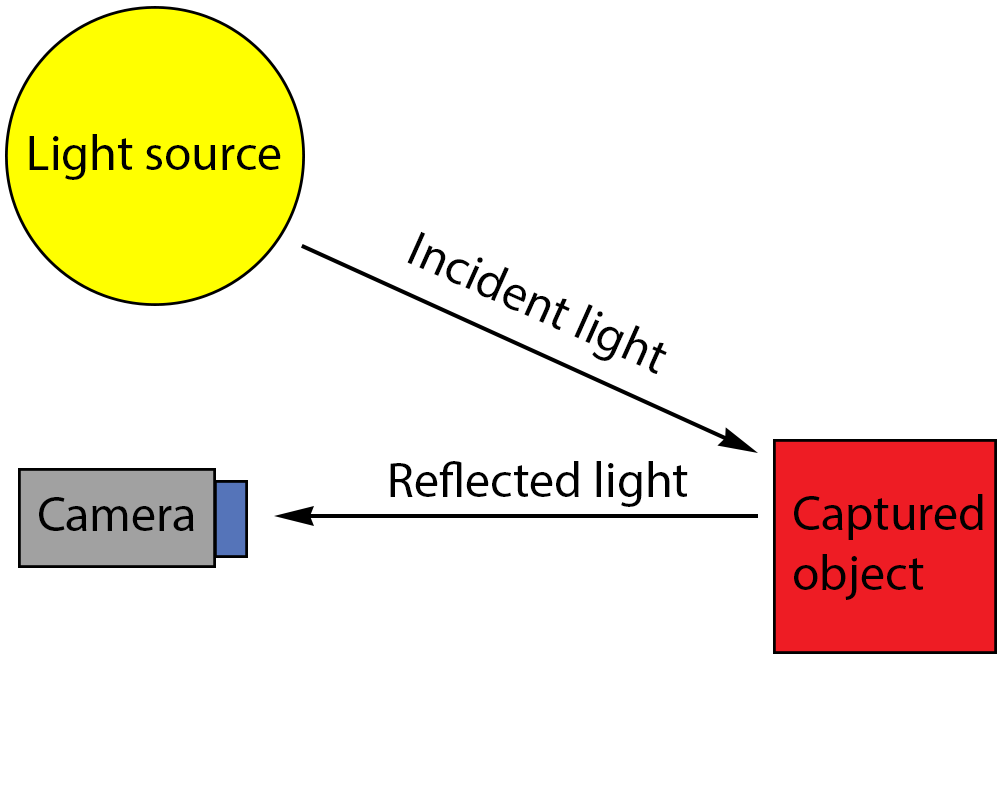
\includegraphics[width=0.5\textwidth]{Pictures/Theory/light_from_sun.png} 
\caption{Light as captured by a camera} 
\label{fig:light_cam} 
\end{figure} 


